\chapter{Results}

\section{Overall MMD behaviour}

Surprisingly, we found that the behaviour of MMD was not as inconsistent for the
types of graphs extracted from proteins as was found on synthetic graphs by
\cite{o2021evaluation}. Figure \ref{fig:mmd_consistent_eps} exhibits a typical
trajectories of MMD values as different perturbation types are progressively
added to $\varepsilon$-graphs with $\varepsilon$ set to $8$\si{\angstrom}. We
can see that both the Spearman and Pearson correlation coefficients averaged
across runs are high, indicating a high correlation between the amount of
perturbation and the normalized MMD values. There is, however, an exception: the
MMD obtained from the degree histogram does not behave as expected, and is very
sensitive to the addition of edges and decreases in value as more and more edges
are added. We expect that this pathology is not very common in real models and
that this can be easily detected manually.

The overall influence of the kernel on MMD's behaviour subject to perturbations
such as Gaussian Noise, can be seen in Figure \ref{fig:mmd_effect_kernel}. We
can see that for low values of $\sigma$ (the hyperparameter of the Gaussian
kernel, see Section \ref{sec:kernels}) and for the linear kernel, MMD values
behave as desired. However, unpredictable patterns emerge when increasing
$\sigma$ and the kernel matrices can ``saturate'' quite easily. This can have
quite unpredictable behaviours: in the case of the degree histogram or the
clustering histogram, this results in an overly sensitive kernel, while the
clustering histogram remains oblivious to large amounts of perturbation.

$k$-NN graphs seem to behave similarly to $\varepsilon$-graphs, in that they are
able to detect perturbations - see Figure \ref{fig:mmd_k_nn_graphs} for an
example with 2-NN graphs. However, they are extremely sensitive to Gaussian
noise and to the addition of edges (see upper left and upper mid pane of Figure
\ref{fig:mmd_k_nn_graphs}). Presumably, this is because very small amounts of
noise ($<4$\si{\angstrom}) affect the direct local neighbourhood of each node
very significantly in such a way that the resulting $k$-NN graph is rapidly
disrupted, which is not necessarily the case with other perturbations. We note
that overall the $\varepsilon$-graphs behave more consistently than $k$-NN
graphs, with 13 out of 21 Pearson's correlation coefficients being higher in
$\varepsilon$-graphs compared to $k$-NN graphs and 11 out of 21 Spearman's
correlation coefficients being higher in 8\si{\angstrom}-graphs compared to 2-NN
graphs. Even when the $\varepsilon$-graphs did not compare favourably, it was by
a considerable lower margin than $k$-NN graphs in a similar setting. This effect
seems to be mitigated by increasing $k$, but this comes at the cost of a lower
Spearman correlation coefficient, which is even less desirable - see Figure
\ref{fig:k_vs_turbulence_gaussian_noise}. Changing kernel parameters did not
alleviate the pathologies (see Supplementary Figure
\ref{fig:mmd_effect_kernel_knn}) and had the same overall effect as observed in
Figure \ref{fig:mmd_effect_kernel}. We therefore proceed with further analysis
using $\varepsilon$-graphs.


\begin{figure}
  \centering
  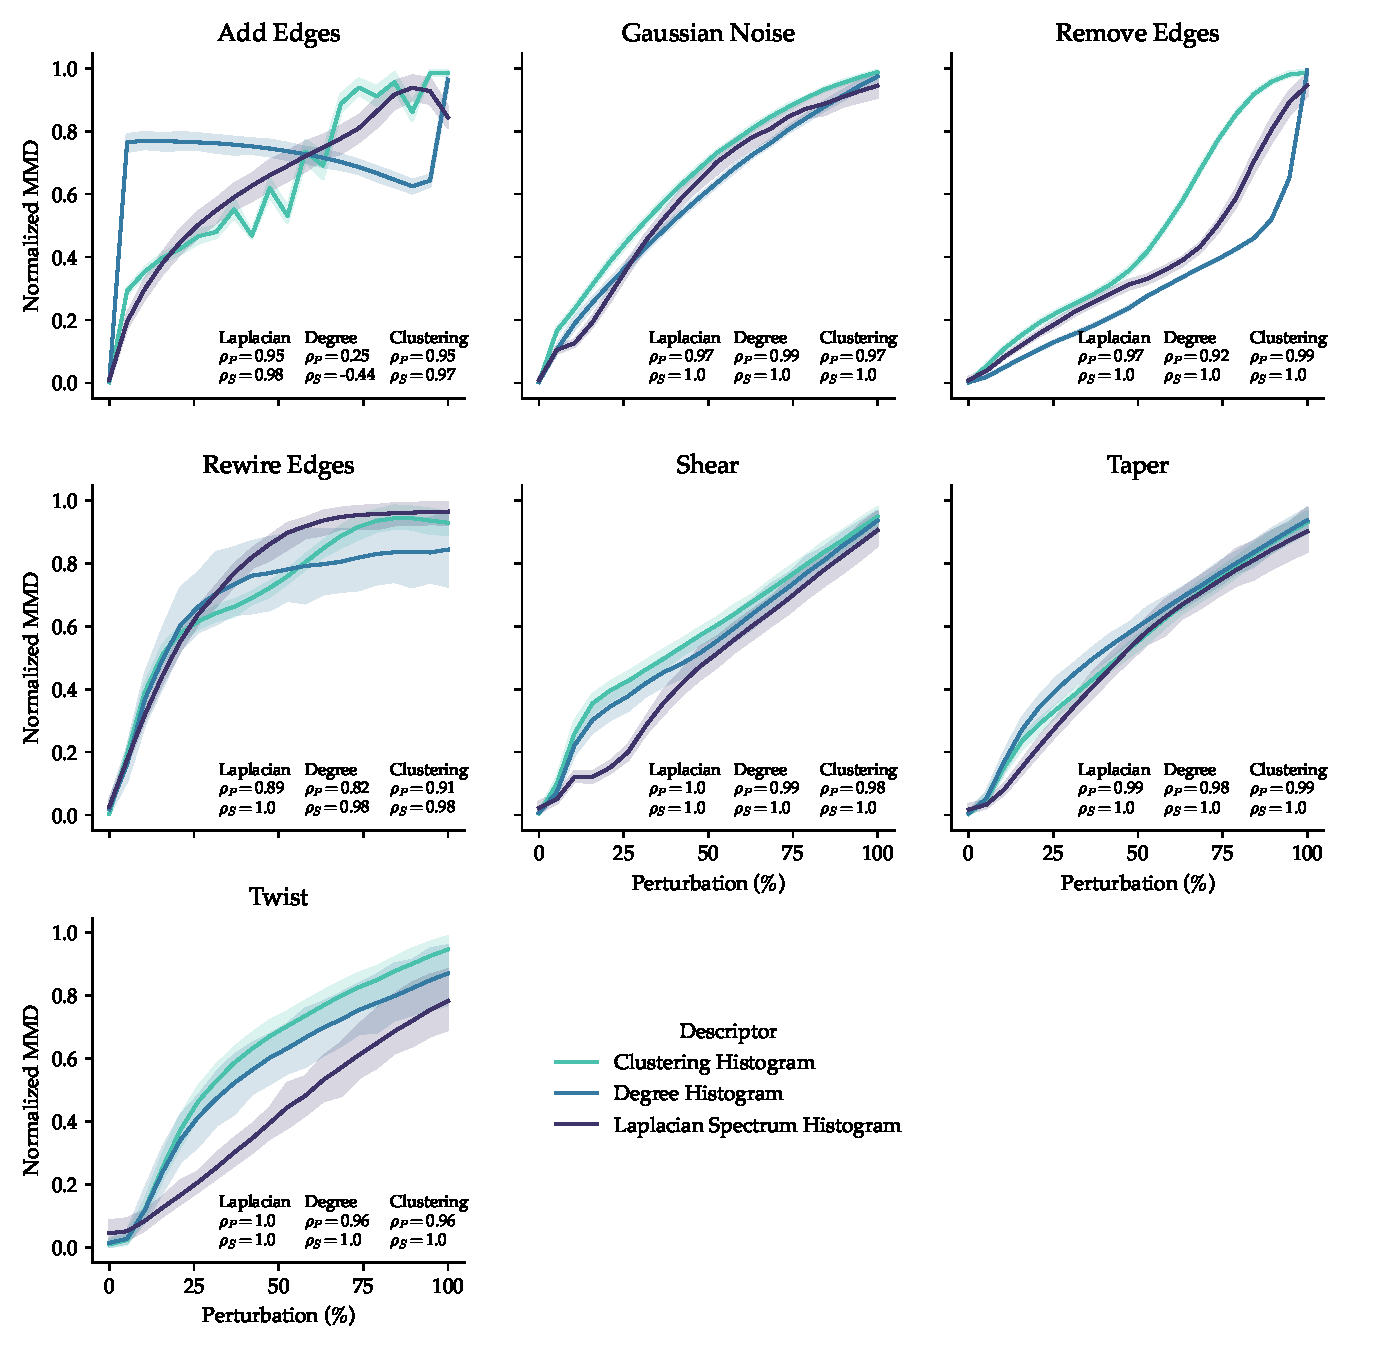
\includegraphics[width=\textwidth]{./figures/results/res_1_1.pdf}
  \caption{MMD vs. perturbation (in \%) for various graph descriptors of the 8\si{\angstrom}-graphs under different perturbations regimes. The kernel
    used to obtain these graphs is the RBF Kernel with bandwidth 0.01.
    $\rho_{S}$: average Spearman correlation coefficient across runs.
    $\rho_{P}$: average Pearson correlation coefficient across runs.}
  \label{fig:mmd_consistent_eps}
\end{figure}


\begin{figure}
  \centering
  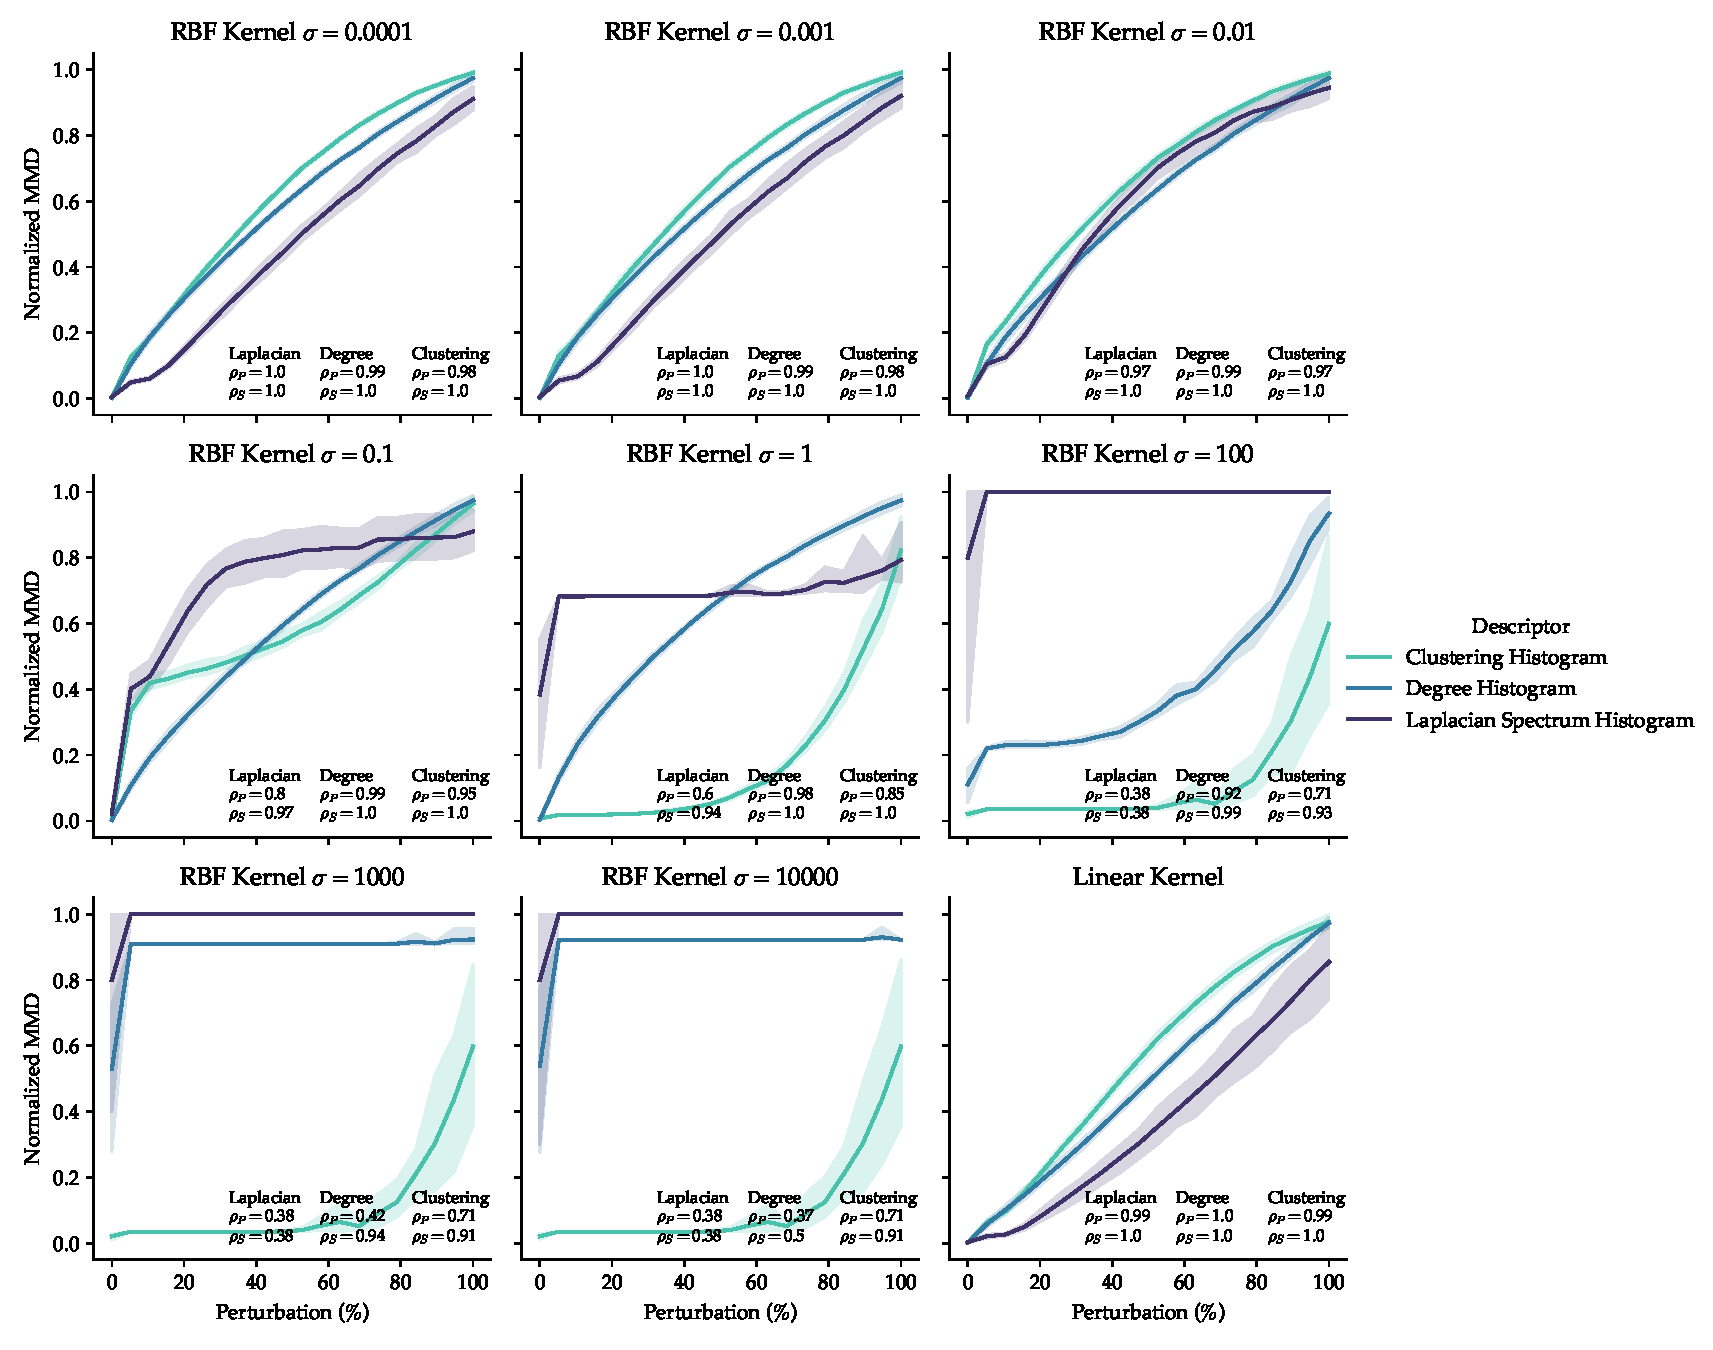
\includegraphics[width=\textwidth]{./figures/results/res_1_2.pdf}
  \caption{MMD vs. Gaussian noise Perturbation (in \%) for various graph descriptors of the
    8\si{\angstrom}-graphs. The kernel here is shown on top of each subplots.}
  \label{fig:mmd_effect_kernel}
\end{figure}

\begin{figure}
  \centering
  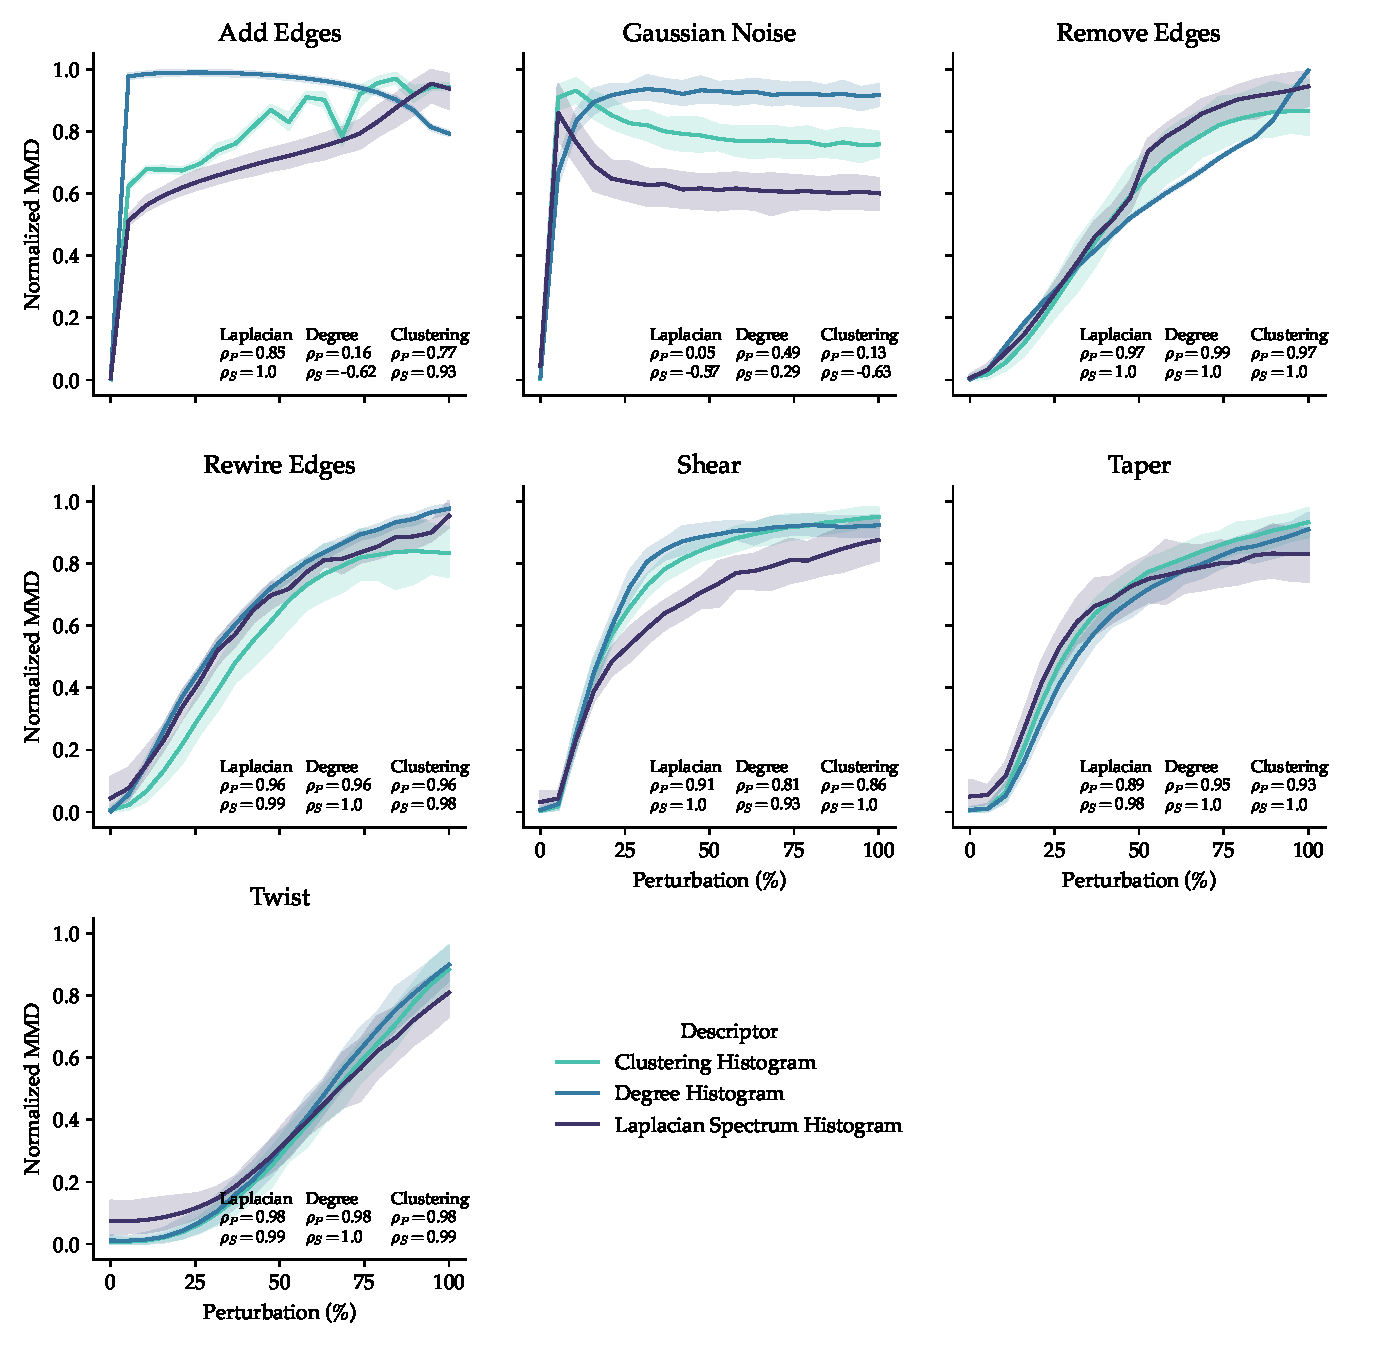
\includegraphics[width=\textwidth]{./figures/results/res_1_3.pdf}
  \caption{MMD vs. Gaussian noise Perturbation (in \%) for various graph descriptors of the
    2-nearest-neighbour graphs.}
  \label{fig:mmd_k_nn_graphs}
\end{figure}

\begin{figure}
  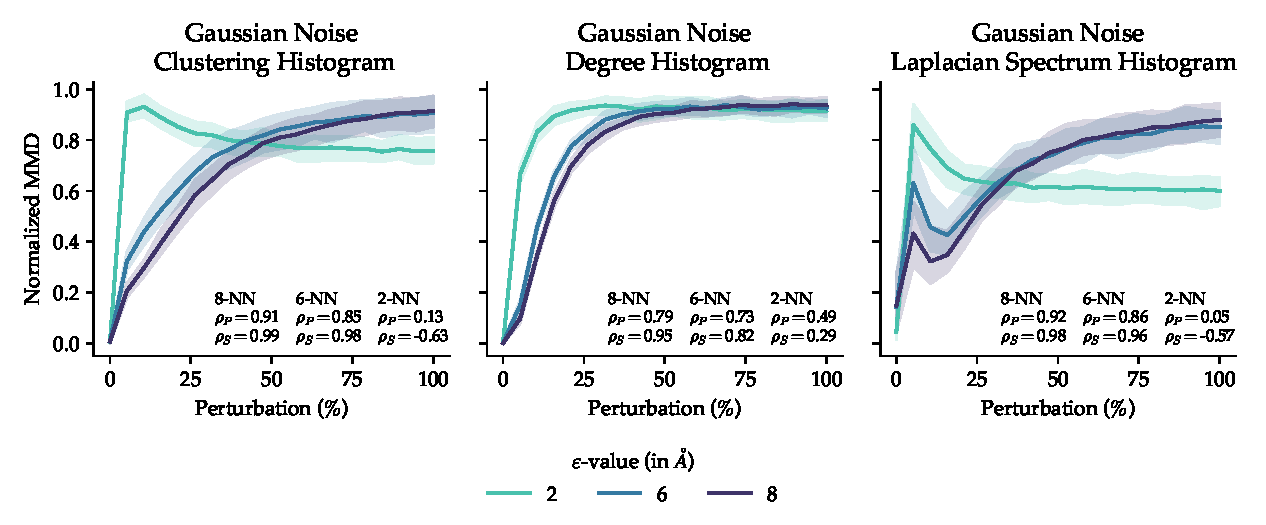
\includegraphics[width=\textwidth]{./figures/results/res_1_4.pdf}
  \caption{MMD vs. Gaussian noise Perturbation (in \%) for various graph
    descriptors and values of $k$ used to extract the $k$-NN graph.}
  \label{fig:k_vs_turbulence_gaussian_noise}

\end{figure}

% MMD is quite stable, somewhat contradicts what obray is saying. Maybe due to
% the different nature of the graphs.

\section{Influence of the graph representation on the sensitivity to perturbations}\label{sec:results_sensitivity}

In the last section, we discussed the notion of sensitivity of a particular MMD
configuration to perturbations. We explore this idea further here. Specifically,
we investigate the impact of the $\varepsilon$ threshold on the resulting
sensitivity of the MMD configuration to various perturbations affecting the
underlying point cloud. Figure \ref{fig:mmd_sensitivity_eps} shows that, in
general, the lower the $\varepsilon$, the more sensitive the MMD to
perturbations. A low sensitivity to perturbation might be useful in the early
stages of modelling, when generated samples only need to \emph{coarsely} match
the reference samples. Conversely, a higher sensitivity to perturbations might
be useful when trying to \emph{finely} distinguish a set of anomalous samples
from the reference samples. Additionally, we can see that under the Gaussian
noise, twisting and tapering perturbation, larger values of $\varepsilon$
introduce larger variations in MMD values.

\begin{figure}
  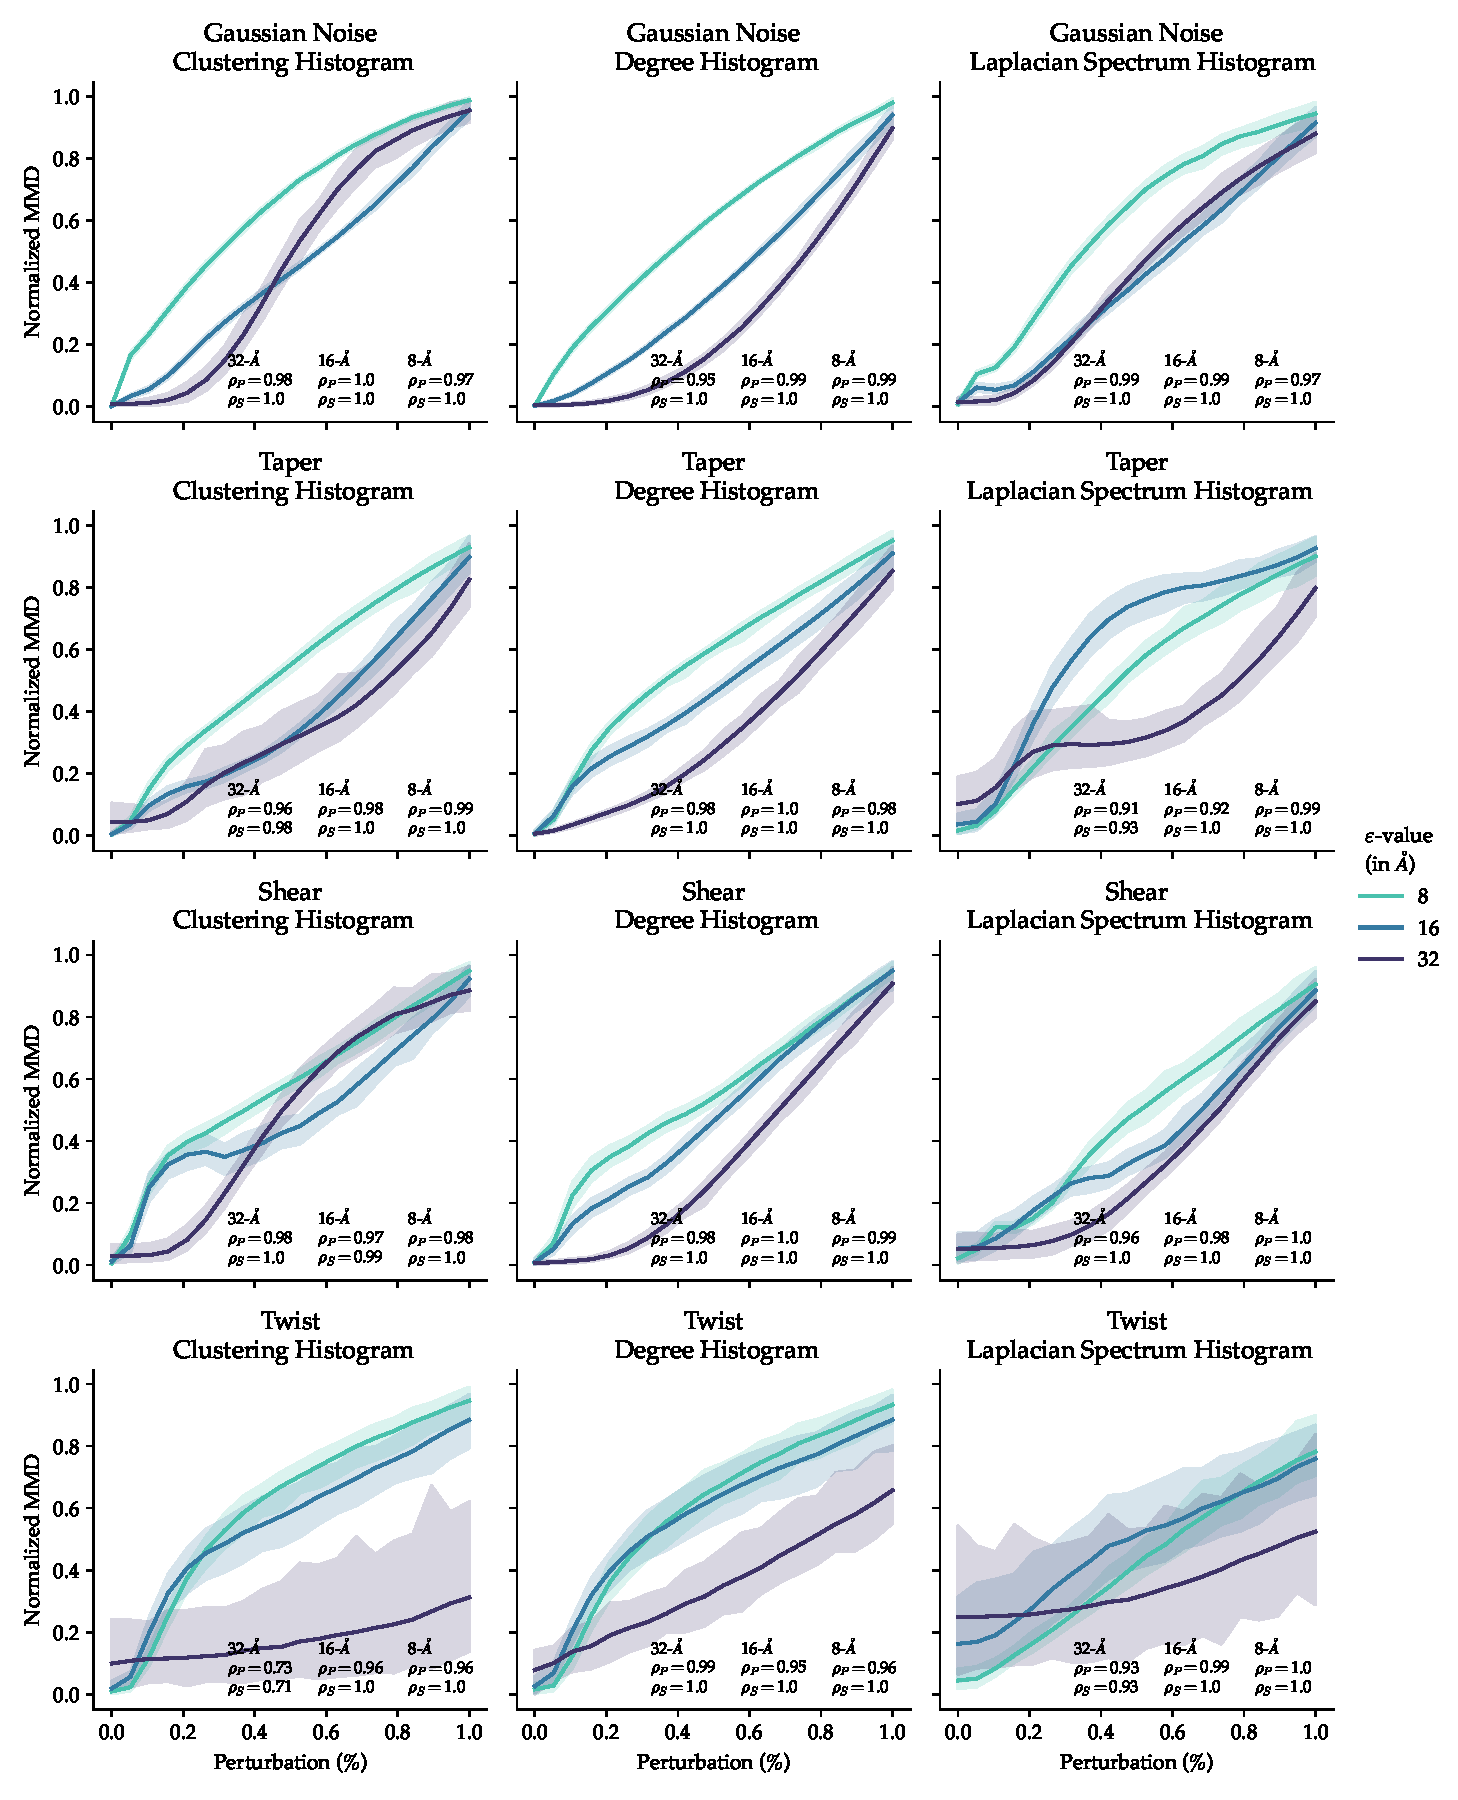
\includegraphics[width=\textwidth]{./figures/results/res_2_1.pdf}
  \caption[MMD vs. point cloud perturbation for various descriptors.]{MMD vs. point cloud perturbation for various descriptors. In general,
when graphs are extracted with a lower $\varepsilon$ value, the MMD curve
increases more rapidly. The only exception to this trend is the laplacian
spectrum histogram descriptor under the tapering perturbation. In multiple
instances, we see that increasing the $\varepsilon$ value increases the MMD variance}
  \label{fig:mmd_sensitivity_eps}
\end{figure}

\section{Graph Kernels}\label{sec:results_graph_kernels}

The results of the behaviour of the Weisfeiler-Lehman kernel (see Sections
\ref{sec:kernels} and \ref{sec:methods_kernels}) can be seen in Figure
\ref{fig:wlk}. Contrary to the tendencies observed in Section
\ref{sec:results_sensitivity}, MMDs obtained using the Weisfeiler-Lehmann
kernels on 8\si{\angstrom} graphs are very insensitive to medium levels of perturbations,
and even completely oblivious to rewiring of graphs and generally insensitive to
graph perturbations unless highly perturbed (see upper row of Figure \ref{fig:wlk}). The most likely explanation
is that the diversity of Weisfeiler-Lehman hashes observed within perturbed or
unperturbed samples is relatively high, which makes distinguishing between the
two a high threshold to overcome. This drawback could dissapear if one is working on
a more targeted set of morphologically similar proteins with a lower diversity
of Weisfeiler-Lehman hashes, but this is beyond the scope of the thesis.

\begin{figure}
  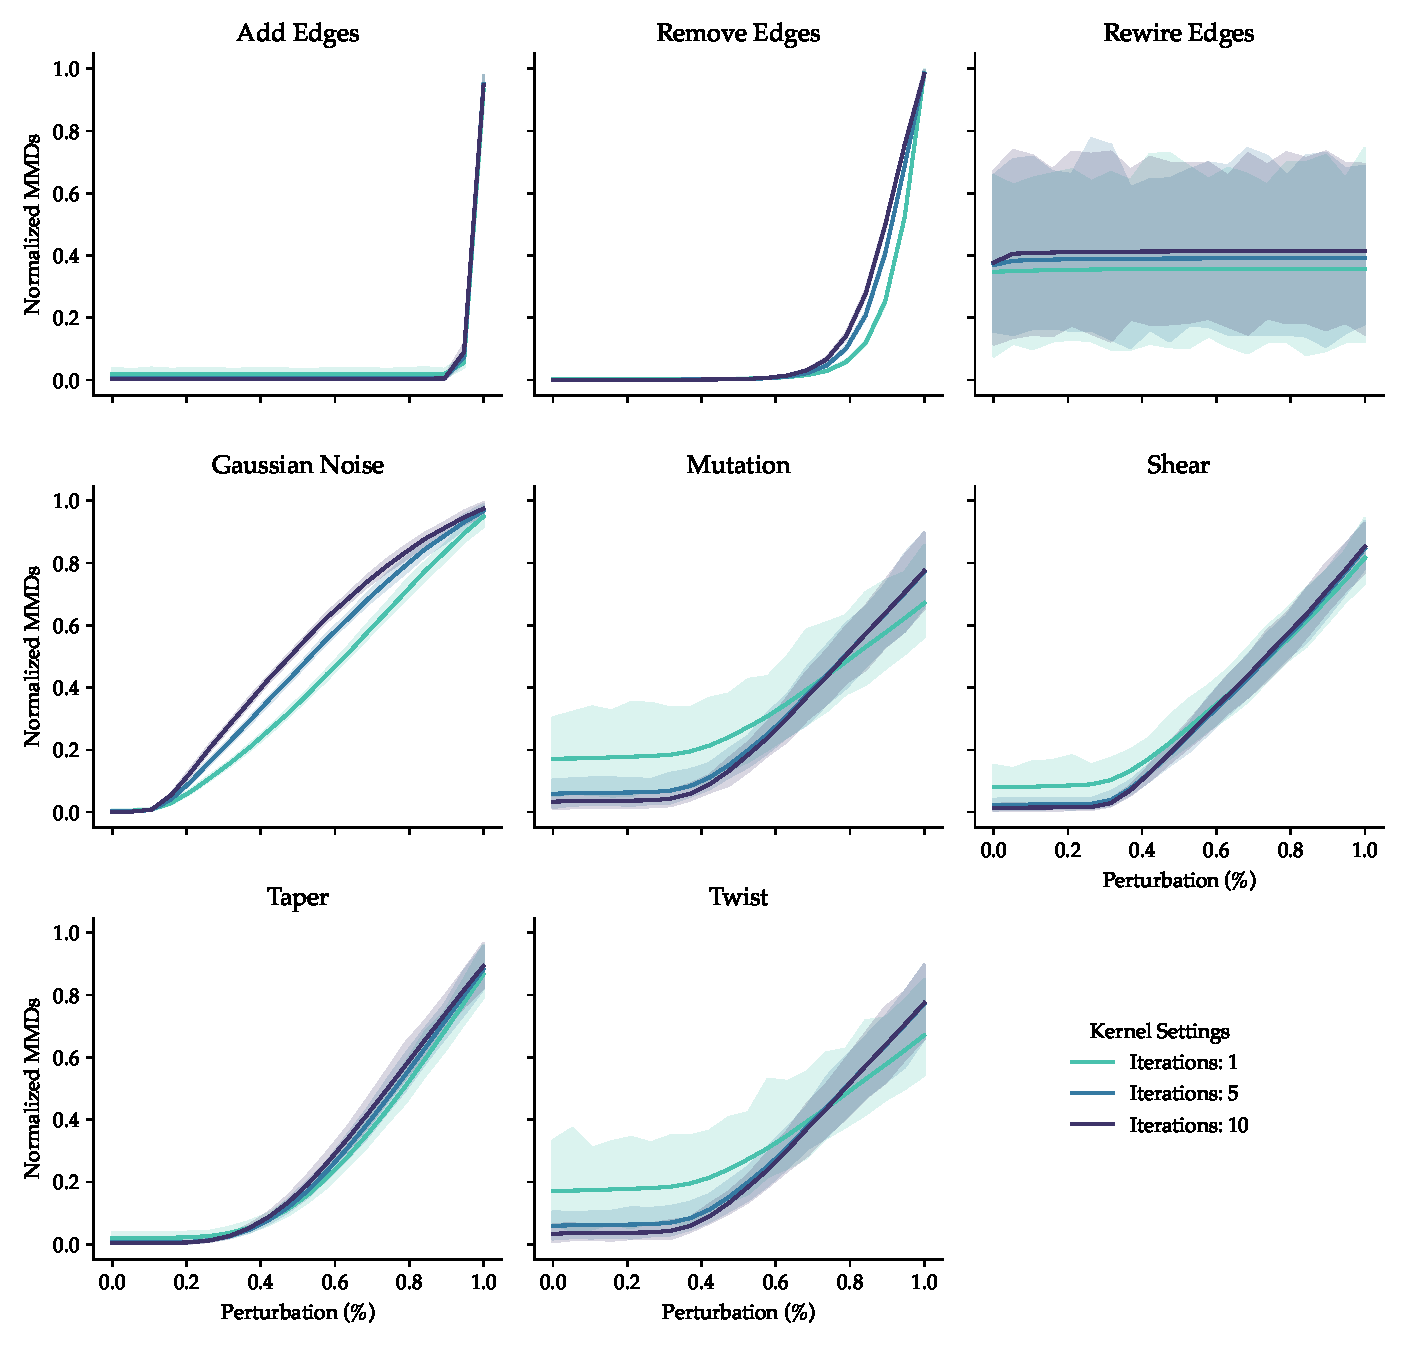
\includegraphics[width=\textwidth]{./figures/results/res_3.pdf}
  \caption[MMD vs. perturbations using the Weisfeiler-Lehman kernel.]{MMD vs.
    perturbations using the Weisfeiler-Lehman kernel using the
    8\si{\angstrom}-graphs as inputs.}
  \label{fig:wlk}
\end{figure}

\section{Protein-specific descriptors}

The behaviour of MMD values derived from the protein-specific descriptor
functions described in section \ref{sec:descriptors} are shown in Figure
\ref{fig:protein_specific_descriptors}. The dihedral angles descriptor is
extremely sensitive to any kind of Gaussian noise, and even decreases in value
when the kernel is not parametrized properly when increasing the shearing. This
is overall a good sign, as it will flag proteins that are unrealistic. The
interatomic distance histogram also behaves well. However, it shows high
variance when twisting the protein, presumably because the intra-sample variance
in distances is a threshold hard to overcome. This phenomenon can also be
noticed in Figure \ref{fig:wlk} with the Weisfeiler-Lehman kernel, and could
dissapear when working on morphologically similar proteins as highlighted in
Section \ref{sec:results_graph_kernels}. Another attractive aspect of this class
of descriptors is that they are very cheap to compute -- see further results in
Section \ref{sec:results_runtime}.

\begin{figure}
  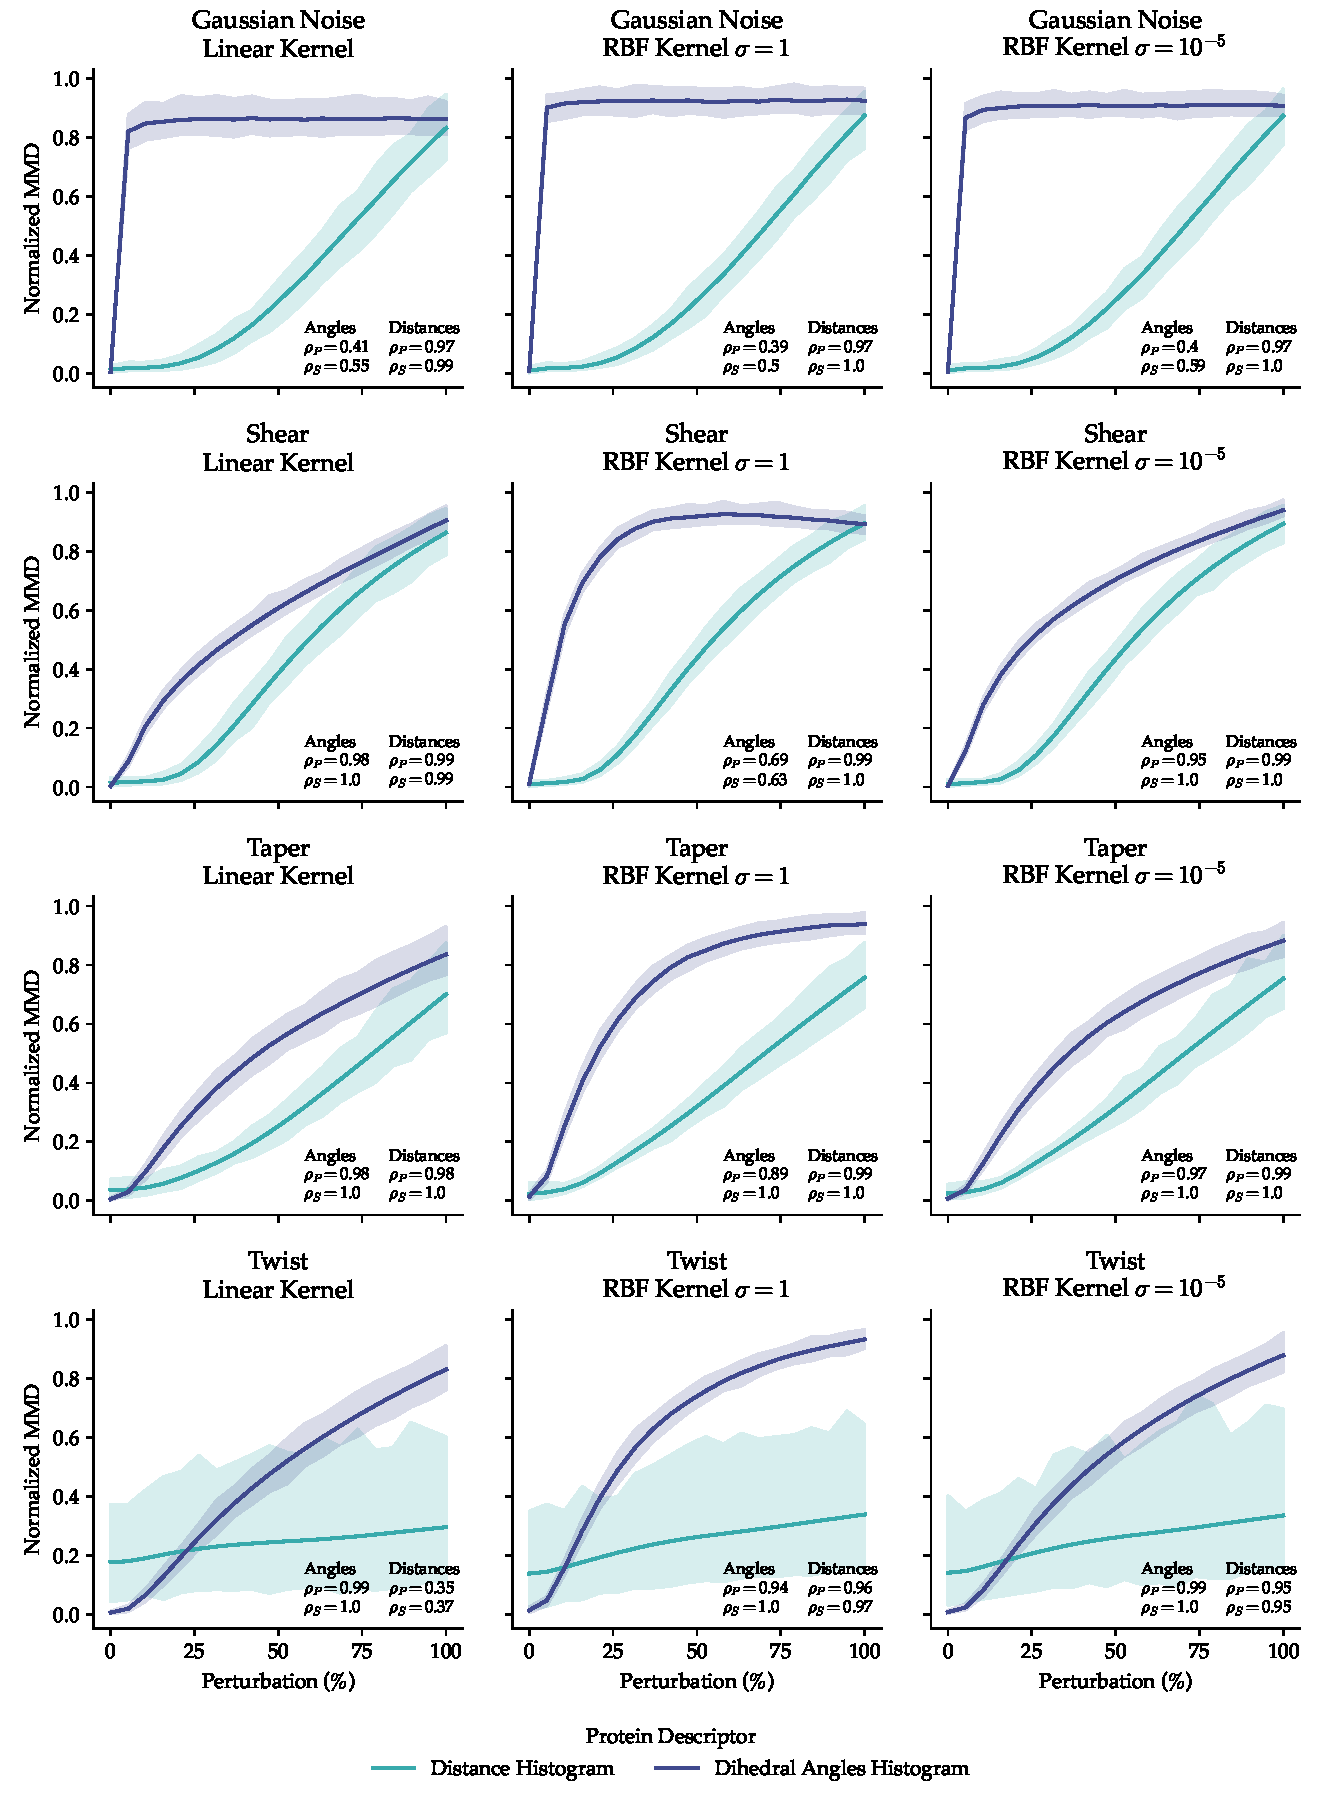
\includegraphics[width=\textwidth]{./figures/results/res_4.pdf}
  \caption[MMD vs. perturbations using the two novel protein descriptors.]{MMD vs. perturbations using the two novel protein descriptors shown
    in Section \ref{sec:descriptors}. Various kernel configurations are shown
    here.}
  \label{fig:protein_specific_descriptors}
\end{figure}

\section{MMD from Learned Embeddings}

Because the only constraint of the input vectors to the kernels accepting
fixed-length vectors as inputs is that they are in $\R$, we can input
fixed-length vector embeddings into them, leveraging the immense progress made
in the past decade regarding embeddings of structured data, specifically protein
sequences. As highlighted in Section

\section{Topological descriptors and kernels}

\section{Runtime}\label{sec:results_runtime}

One of the desiderata of MMD is a low computational complexity (see Section
\ref{sec:evalproblem}). As such, we report the various computation times for
each of the important elements of the pipelines outlined in this thesis. The
summary of all execution times can be found in Table \ref{tab:runtimes}.


\begin{table}
  \centering
  \begin{tabular}{lll}
    \toprule
    \textbf{Operation} &  \textbf{Execution Time} \\
    \midrule
    Vietoris-Rips Filtration & \\
    ESM Embedding & \\
    Degree Distribution Histogram & \\
    Clustering Coefficient Histogram & \\
    Laplacian Spectrum Histogram & \\
    \bottomrule
  \end{tabular}
  \caption{Runtime and computational complexity of the various elements of the pipeline.}
  \label{tab:runtimes}
\end{table}


% Scale FREE!!

% \section{Fixed-Length Vectors}

% \subsection{Domain agnostic descriptors}

% \subsection{Protein-specific descriptors}

% \subsection{Embeddings}

% \section{Graph Kernels}

% \subsection{Weisfeiler-Lehmann}

% \section{Topological Representations and Kernels}

% \subsection{Persistence Fisher Kernel}

\section{Summary}
